\documentclass{ctexart}
\usepackage{amsmath}
\usepackage{graphicx} % Required for inserting images
\usepackage{lipsum}
\usepackage{geometry}
\usepackage{fancyhdr}
\usepackage{lastpage}
\usepackage{placeins}
\usepackage{subcaption}
\usepackage{float} 
\usepackage{amsthm}
\usepackage{amssymb}
\usepackage{array}
\usepackage{booktabs}
\usepackage{tabularx}\usepackage{tabularx}
\usepackage{booktabs, longtable}
\newcommand{\keywords}[1]{\par\noindent\textbf{关键词：} #1}
\renewenvironment{abstract}
 {\par\large\begin{center}\textbf{\large\abstractname}\end{center}\par\noindent\ignorespaces}
 {\par}
\geometry{left=2.5cm,right=2.5cm,top=2cm,bottom=2cm}
\pagestyle{fancy}
\fancyhf{}

\rhead{ }
\cfoot{第 \thepage 页 （共 \pageref{LastPage} 页）}

\title{题目}
\author{曹建宇 \and 李正阳 \and 朱睿杰}
\date{\today}
\newtheorem{theorem}{定理}[subsection]   % 定理按节编号
\newtheorem{lemma}[theorem]{引理}     % 引理与定理共用计数器
\newtheorem{definition}{定义}[subsection]   % 定义按节编号
\newcommand{\Teff}{T_{\text{eff}}}
\begin{document}
\maketitle 
\begin{abstract}  % 摘要
这是一段摘要
\end{abstract}
\keywords{关键词1，关键词2，关键词3}  % 关键词
\newpage

\tableofcontents
\newpage
\section{问题重述} 
\subsection{问题背景}
在现代防空作战中，空地导弹凭借高精度、高速度对地面重要目标构成严重威胁。而烟幕干扰作为一种软防护措施，通过化学燃烧或爆炸分散形成烟幕或气溶胶云团在来袭导弹视线上形成遮蔽云团，可有效干扰敌方导弹，具有低成本高收益的特点，逐渐成为现代军事中防空的主流选择之一。而无人机的发展，使得烟幕弹的投放范围更加广阔，从而使得精准投放烟幕弹以达到最大遮蔽效果成为可能。

然而，无人机飞行的方向和速度，以及烟幕弹应在何处投放、应当延迟几秒起爆，极大影响最终的遮蔽效果。实际作战中，烟幕弹的下降、敌方导弹的高速移动等，使得实际的遮蔽时间非常短暂。如何通过优化，确定无人机的移动方向、移动速度以及烟幕弹投放地点、延迟起爆时间，以达到遮蔽效果的最大化，成为军事专家必须研究的课题。
\subsection{问题提出}
现已知真目标和假目标的位置和形状，三枚来袭导弹和五架无人机的坐标，以及一些运动参数，本文需要通过数学建模解决以下问题：

\textbf{问题一：}针对单架无人机，已知其运动方向、投放地点和延迟起爆时间，通过建立模型确定其仅投掷一枚烟幕弹，对一运动方向、速度固定的导弹的遮挡效果。

\textbf{问题二：}针对单架无人机，同样研究其投掷一枚烟幕弹的情形，对其飞行方向、飞行速度、烟幕干扰弹投放点、烟幕干扰弹起爆点进行优化，使得遮蔽时间最长。

\textbf{问题三：}针对单架无人机可投放多枚烟幕弹的情形，通过优化，使得其对单枚导弹的遮蔽时间最长。

\textbf{问题四：}不溶于问题三一机多弹的情形，考察三架无人机，各投放一枚烟幕弹，通过三架无人机在三维空间中的配合协调实现对于导弹的最佳屏蔽效果。

\textbf{问题五：}将问题推广到三架无人机、每架无人机最多投放三枚的情形，需要同时解决任务分配（哪架无人机干扰哪一枚导弹）和资源调度（各飞机投几枚，何时投，何时起爆）的问题。
\section{问题分析}
\subsection{问题一}
问题一是基础情况，要求计算在给定参数下烟幕干扰弹对导弹M1的有效遮蔽时长。首先可以利用题目给定的参数算出烟幕弹起爆时刻烟幕弹和导弹的位置作为后续模型的初值，之后需要根据空间几何的知识找到满足使有效遮挡这一要求成立的几何关系，最后就可以根据初值和该几何关系从起爆时刻进行变步长搜索找出满足有效遮挡的时间范围。
\subsection{问题二}
问题二不同于问题一在给定的参数下求解，而是需要延用问题一的分析，把无人机航向速度、烟幕弹投放、引爆时间四个参数作为决策变量，以最大化有效遮挡时间作为目标函数建立单机单弹情况下的策略优化模型，在满足一些物理约束、运动学约束、边界条件的情况下求解出烟幕弹的最优投放策略。
\subsection{问题三}
问题三基于问题二的优化模型，需协调多枚烟幕弹的投放与起爆时序，避免时间重叠或遗漏，通过时序优化与协同控制延长总有效遮蔽时间。由于三枚烟幕弹是由同一无人机发射，其在空间上位置相差不远，考虑有效遮挡时，可能会存在单个云团不能有效遮挡，而多个云团在时间上交替覆盖时形成连续有效遮挡的情况。
\subsection{问题四}
问题四是多机单弹拦截同一目标的情况，与问题三的单机多弹模式不同，问题四的核心在于多无人机之间的空间协同和时间协调，这里不需要考虑投弹时间间隔，但是三枚烟幕弹爆炸产生的云团应该避免在空间上过度重叠，同时时间上要保持连续。这需要建立多烟幕弹协同遮蔽的判定模型，分析多个云团在空间上的遮蔽效果叠加关系，在考虑各无人机独立决策的前提下，通过协同目标函数确保整体遮蔽效果最大化。
\subsection{问题五}
问题五是最一般化的情形，涉及5架无人机、每架至多3枚烟幕弹，同时对抗3枚来袭导弹。该问题的复杂度显著增加，需同时处理多机、多弹、多目标的分配与协同问题。核心难点在于：一方面要为每枚导弹分配合适的烟幕弹资源，另一方面要使得所有导弹在同一时刻均被至少一个云团遮蔽的时间区间尽可能长。决策变量包括各无人机的飞行方向与速度、每枚弹的投放时机和起爆延迟，以及弹与弹之间的分配关系。这属于混合整数非线性规划问题，需要建立统一的遮蔽时间并集（针对单目标）或交集（针对多目标同时遮蔽）的目标函数，并采用启发式优化算法求解全局较优的投放策略。
\section{模型假设}
\begin{enumerate}
    \item 为简化研究，我们仅研究无风情况的遮蔽，不考虑空气阻力对运动的影响。
    \item 导弹、无人机、烟幕弹、假目标均视为质点进行运动学研究。
    \item 烟幕弹起爆后瞬时膨胀成一个半径为$10m$的球，并且在有效持续时间$(20s)$内不扩散，烟雾遮蔽能力不变。
\end{enumerate}
\section{符号说明}
\begin{longtable}{@{} p{2.8cm} p{6.5cm} p{1.8cm} @{}}
% ========== 第一页的表头 ==========
\caption{导弹与烟幕弹相关符号定义}
\label{tab:symbols} \\
\toprule
\textbf{符号} & \textbf{含义} & \textbf{单位} \\
\midrule
\endfirsthead


\multicolumn{3}{c}{接上页} \\
\toprule
\textbf{符号} & \textbf{含义} & \textbf{单位} \\
\midrule
\endhead


\bottomrule
\multicolumn{3}{r}{续下页} \\
\endfoot


\bottomrule
\endlastfoot


$O_d$          & 假目标位置（原点）                                 & m \\
$O_1$          & 真目标底面圆心位置                                     & m \\
$r$            & 圆柱体半径                                             & m \\
$h$            & 圆柱体高度                                             & m \\
$\mathbf{M}(t)$ & 导弹位置向量（时刻 $t$）                             & m \\
$V_M$          & 导弹速度大小                                           & m/s \\
$\hat{\mathbf{u}}_m$ & 导弹飞行方向单位向量                                   & -- \\
$T_{\text{end}}$ & 导弹到达假目标总飞行时间                             & s \\
$\mathbf{F}_1(0)$ & 无人机初始位置                                     & m \\
$V_{\text{drone}}$          & 无人机速度大小                                         & m/s \\
$\mathbf{u}_f$ & 无人机水平方向单位向量                                 & -- \\
$t_{\text{rel}}$ & 烟幕弹投放时刻                                     & s \\
$\mathbf{R}_\text{pt}$   & 烟幕弹投放点位置                                       & m \\
$t_{delay}$ & 起爆延时                                     & s \\
$t_{\text{det}}$ & 烟幕弹起爆时刻                                     & s \\
$\mathbf{A}_{\text{det}}$ & 烟幕弹起爆点位置                             & m \\
$\mathbf{A}(t)$ & 烟幕球心位置（时刻 $t$）                           & m \\
$v_s$          & 烟幕云团下沉速度                                       & m/s \\
$T_{\text{life}}$ & 烟幕有效持续时间                                   & s \\
$R_s$          & 烟幕球半径                                             & m \\
$\pi_{\mathbf{M}}(\mathbf{P})$ & 以导弹为中心的球面投影映射                   & -- \\
$\Omega_C(\mathbf{M})$ & 圆柱体在导弹视角下的投影区域     & -- \\
$\Omega_B(\mathbf{M},\mathbf{A})$ & 烟幕球在导弹视角下的投影球冠               & -- \\
$\mathbf{u}_A$ & 球冠中心方向单位向量                                   & -- \\
$\alpha$       & 球冠半角                              & rad \\
$\theta_{\max}$ & 圆柱投影区域到球冠中心的最大角距离                  & rad \\
$T_{\text{eff}}$ & 有效遮蔽总时长                                     & s


\end{longtable}
\section{模型准备}
\subsection{建系}
根据题意，我们以假目标为原点，建立空间直角坐标系，下图为初始坐标图。
\begin{figure}[H]
    \centering
    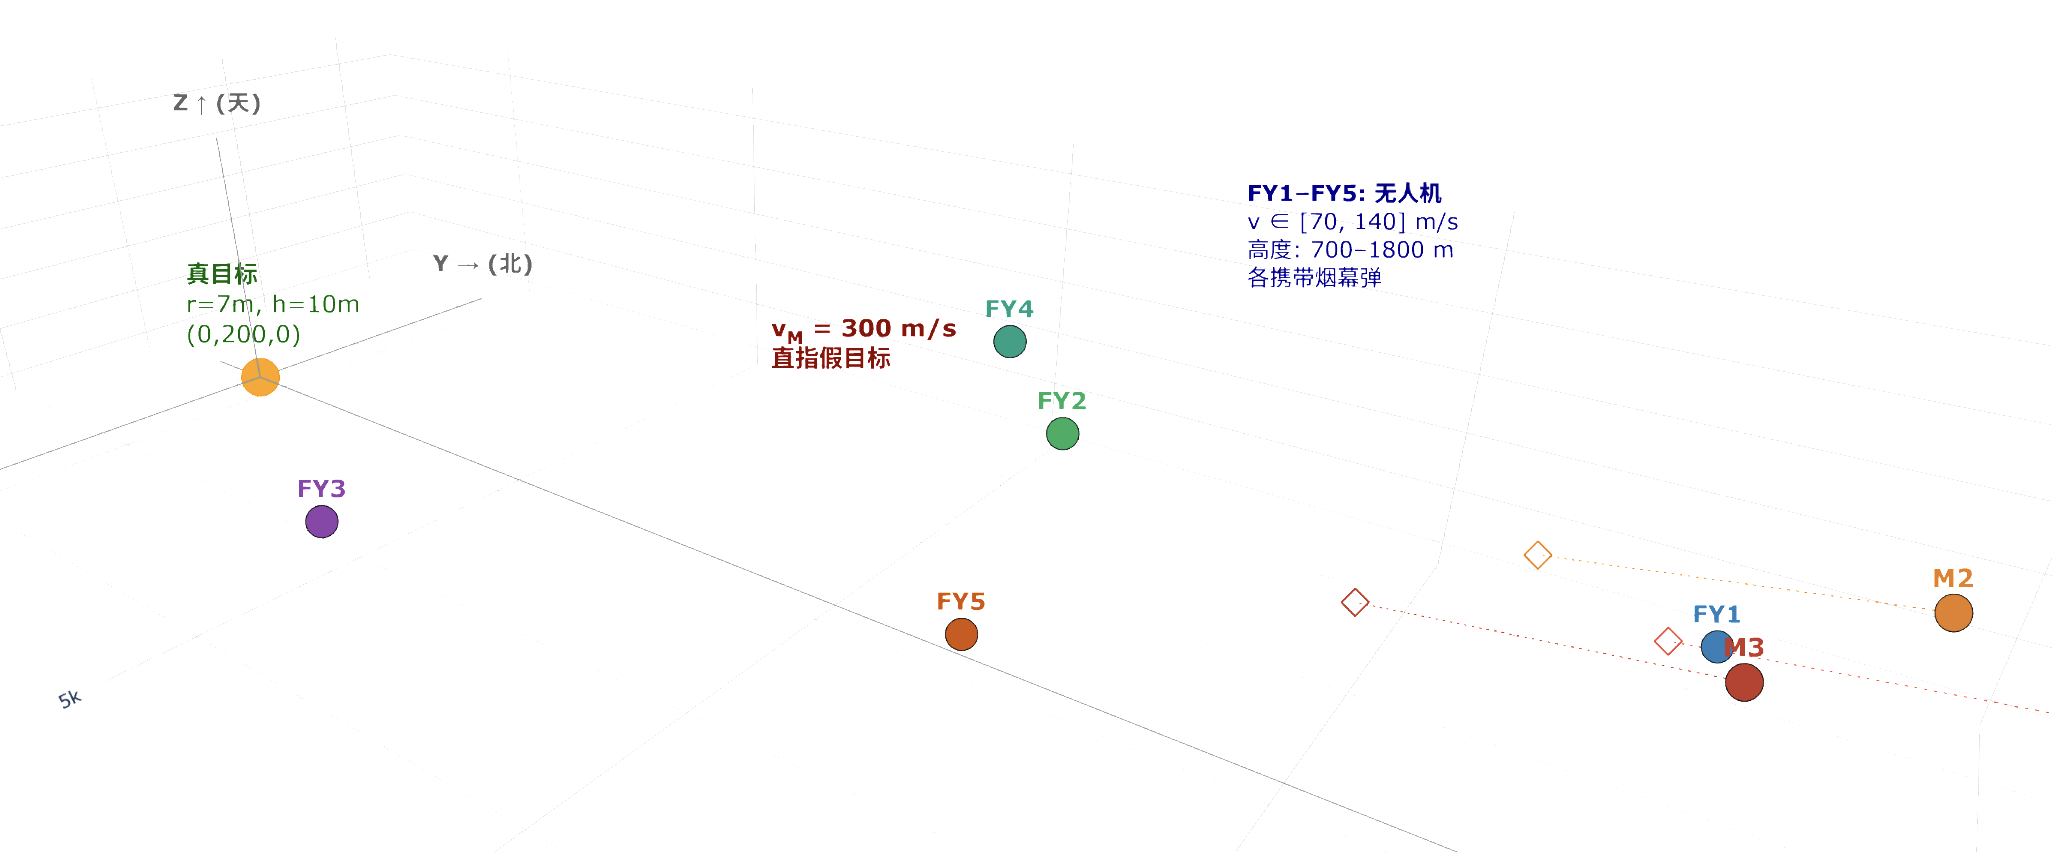
\includegraphics[width=0.8\textwidth]{20260803185247_339_649.png}
    \caption{初始坐标图}
    \label{fig:initial_coords}
\end{figure}
\subsection{无人机抛弹与烟幕运动}

无人机在高度 $H$ 处以恒定速度 $V_{\text{drone}}$ 沿方向角 $\theta$（以 $+X$ 轴为 $0^\circ$ 逆时针度量）水平直线飞行，全程速度与航向不变。在 $t_{\text{rel}}$ 时刻，无人机投放烟幕干扰弹。投放后，炸弹在水平方向继承无人机的惯性速度继续做匀速直线运动，竖直方向受重力作用做自由落体运动，加速度 $g = 9.8\ \mathrm{m/s^2}$。经 $t_{delay}$ 秒延时后，炸弹起爆，瞬间形成半径 $R_s = 10\ \mathrm{m}$ 的烟幕球体。

记无人机初始位置为 $\mathbf{P}_{\text{FY}} = (x_0, y_0, H)$，其水平方向单位向量为 $\mathbf{u}_f = (\cos\theta, \sin\theta, 0)$，则投放点与起爆点位置分别为：
\[
\mathbf{R}_{\text{pt}} = \mathbf{P}_{\text{FY}} + V_{\text{drone}} \cdot \mathbf{u}_f \cdot t_{\text{rel}}, \qquad
\mathbf{A}_{\text{det}} = \mathbf{R}_{\text{pt}} + V_{\text{drone}} \cdot \mathbf{u}_f \cdot t_{delay} + \left(0,\; 0,\; -\frac{1}{2}g\,t_{delay}^2\right).
\]

起爆时刻 $t_{\text{det}} = t_{\text{rel}} + t_{delay}$。起爆后，烟幕球以恒定速度 $v_s = 3\ \mathrm{m/s}$ 竖直下沉，有效持续时间 $T_{\text{life}} = 20\ \mathrm{s}$。烟幕球心在任意时刻 $t \in [t_{\text{det}},\; t_{\text{det}}+T_{\text{life}}]$ 的位置为：
\[
\mathbf{A}(t) = \mathbf{A}_{\text{det}} - (0,\; 0,\; v_s) \cdot (t - t_{\text{det}}).
\]

在实际优化中（问题二及其后），无人机的飞行参数可由起爆点反推。给定起爆时刻 $t_{\text{det}}$ 和起爆点坐标 $(A_x, A_y, A_z)$，水平位移和自由落体高度唯一确定 $V_{\text{drone}}$ 和 $t_{delay}$：
\[
V_{\text{drone}} = \frac{\sqrt{(A_x - x_0)^2 + (A_y - y_0)^2}}{t_{\text{det}}}, \qquad
t_{delay} = \sqrt{\frac{2(H - A_z)}{g}}, \qquad t_{\text{rel}} = t_{\text{det}} - t_{delay} \geq 0.
\]

该逆向参数化将优化变量从 $(V_{\text{drone}}, \theta, t_{\text{rel}}, t_{delay})$ 等价转换为 $(t_{\text{det}}, A_x, A_y, A_z)$——优化起爆时机和起爆点位置的同时，无人机飞行参数自然确定。

\subsection{遮蔽判断模型}
为了方便理解，我们将遮蔽问题简化为点、球面和圆柱体三者之间的静态位置关系问题。

记导弹所在点为$\mathbf{M}$，起爆后球 $\mathcal{B}$的球心为$\mathbf{A}$，球的张角为$\alpha$，圆柱体 $\mathcal{C}$表面上任意一点为$\mathbf{P}$，则有效遮挡的情形如下图所示：

\begin{figure}[H]
    \centering
    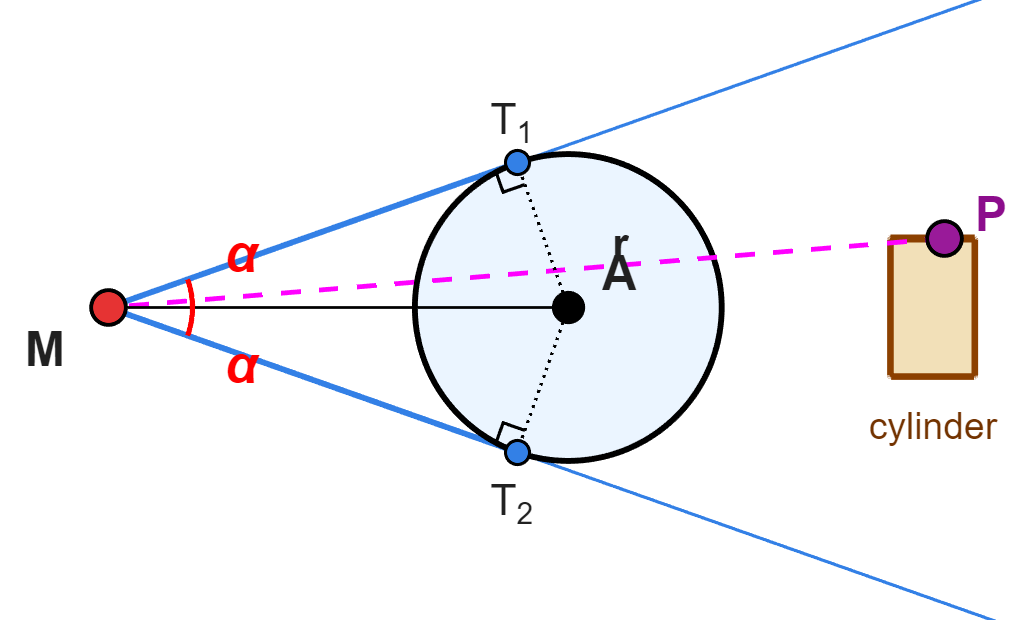
\includegraphics[width=0.8\textwidth]{20260803193802_233_32.png}
    \caption{有效遮挡情况}
    \label{fig:effective_shielding}
\end{figure}
\subsubsection{单位球面映射}
若我们在导弹的位置向量$\mathbf{M}$处作一个单位球面 $\mathbb{S}^2$，我们模拟光线的成像，将圆柱形的轮廓和烟幕球的轮廓均逆着视线的方向投影到$ \mathbb{S}^2$上。如此，我们仅需关注视线的方向，无需关注视线的长度。若这个点为点$P$，则其投影到这个单位球面后的单位向量为
\[
\pi_{\mathbf{M}}(\mathbf{P}) = \frac{\mathbf{P} - \mathbf{M}}{\|\mathbf{P} - \mathbf{M}\|}, \quad \mathbf{P} \neq \mathbf{M}.
\]
\subsubsection{圆柱面的投影}
如果我们从斜上方观察圆柱体的轮廓，我们发现其轮廓可以由四条线组成，从下图可以直观看出：

\begin{figure}[H]
    \centering
    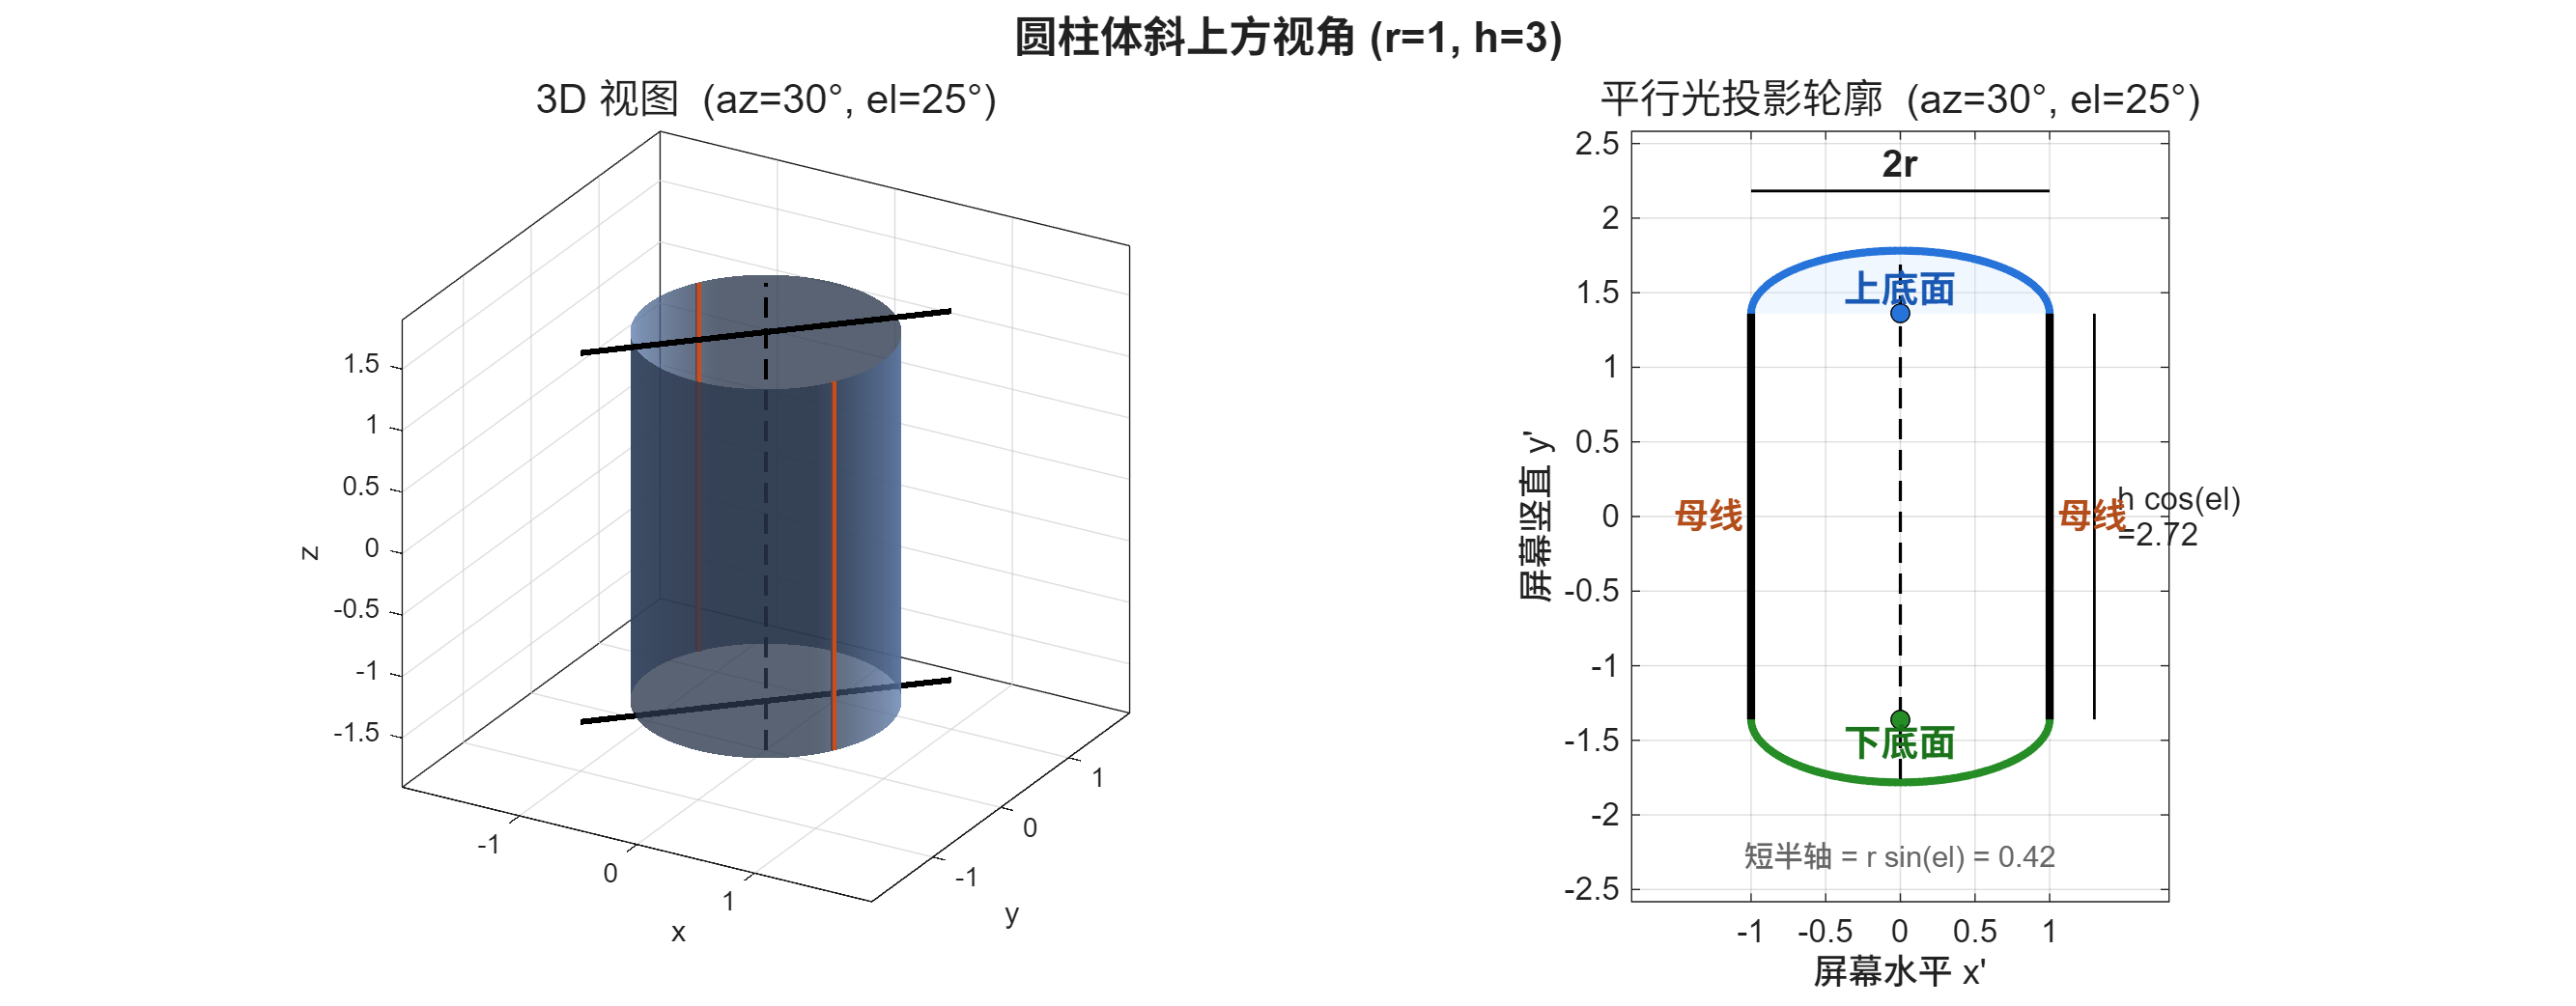
\includegraphics[width=0.8\textwidth]{cylinder_projection.png}
    \caption{圆柱体投影情况}
    \label{fig:cylinder_projection}
\end{figure}


具体如下表所示：
\begin{table}[h]
\centering
\begin{tabular}{c|c|c}
\toprule
边界 & 参数方程 & 说明 \\
\midrule
左切线 $\mathcal{L}_L$ & $\mathbf{T}_L + (0,0,s),\; s\in[0,H]$ & 从 $\mathbf{M}$ 到圆柱的左切线竖线段 \\
右切线 $\mathcal{L}_R$ & $\mathbf{T}_R + (0,0,s),\; s\in[0,H]$ & 右切线竖线段 \\
顶面弧 $\mathcal{E}_{\text{top}}$ & $O_1 + (0,0,H) + r(\cos\phi,\sin\phi,0)$ & 顶面可见椭圆弧 \\
底面弧 $\mathcal{E}_{\text{bot}}$ & $O_1 + r(\cos\phi,\sin\phi,0)$ & 底面可见椭圆弧（远离 $\mathbf{M}$ 的半弧） \\
\bottomrule
\end{tabular}
\end{table}

其中 $\mathbf{T}_L, \mathbf{T}_R$ 是 $\mathbf{M}$ 到圆柱圆周（xy平面）的两切点，切线半角 $\psi = \arcsin(r / d_{xy})$，\\$d_{xy} = \sqrt{(M_x)^2 + (M_y-200)^2}$。\\
圆柱投影区域：
\[
\Omega_{\mathcal{C}}(\mathbf{M}) = \{\pi_{\mathbf{M}}(\mathbf{P}) \mid \mathbf{P} \in \partial\mathcal{C}_{\text{vis}}(\mathbf{M})\}.
\]
实际计算中，对 $\partial\mathcal{C}_{\text{vis}}$ 均匀采样 $N \approx 215$ 个点，得到方向向量集 $\{\mathbf{u}_i\}_{i=1}^{N}$。

\subsubsection{烟幕球投影区域}

烟幕球 $\mathcal{B}(\mathbf{A}, R_s)$ 投影到单位球面上是一个球冠：
\[
\Omega_{\mathcal{B}}(\mathbf{M}, \mathbf{A}) = \left\{\mathbf{u} \in \mathbb{S}^2 \;\middle|\; \arccos(\mathbf{u} \cdot \mathbf{u}_A) \leq \alpha\right\},
\]
其中
\[
\mathbf{u}_A = \pi_{\mathbf{M}}(\mathbf{A}) = \frac{\mathbf{A} - \mathbf{M}}{\|\mathbf{A} - \mathbf{M}\|}, \quad \alpha = \arcsin\left(\frac{R_s}{\|\mathbf{M} - \mathbf{A}\|}\right).
\]
$\mathbf{u}_A$ 为球冠中心方向，$\alpha$ 为球冠半角（烟幕球对 $\mathbf{M}$ 的张角的一半）。

\subsubsection{遮蔽判定}

\begin{definition}
烟幕球 $\mathcal{B}(\mathbf{A}, R_s)$ 完全遮挡圆柱体 $\mathcal{C}$，当且仅当圆柱体的投影区域被烟幕球的投影球冠完全包含，即：
\[
\Omega_{\mathcal{C}}(\mathbf{M}) \subseteq \Omega_{\mathcal{B}}(\mathbf{M}, \mathbf{A}).
\]
\end{definition}
此时情况如下图所示（为方便查看，此处画的并非单位圆）

\begin{figure}[H]
    \centering
    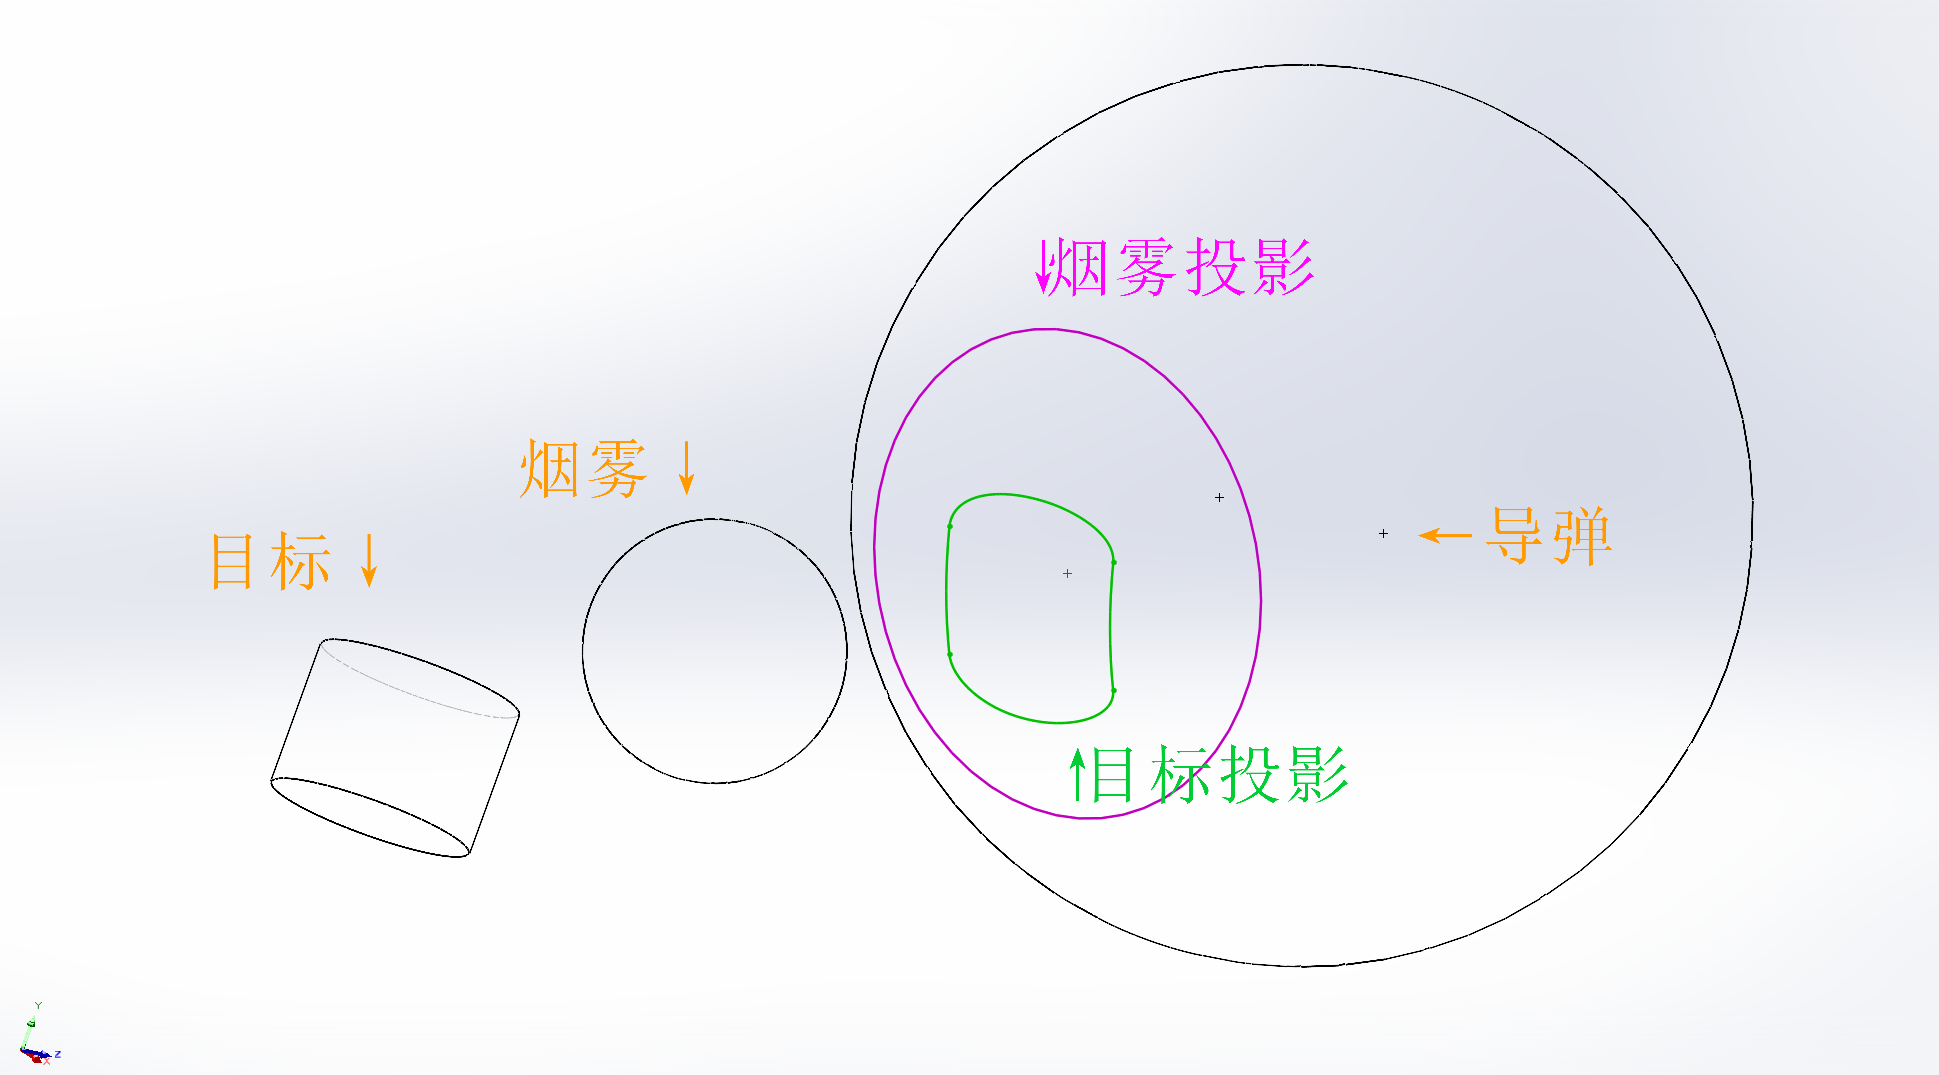
\includegraphics[width=0.8\textwidth]{20260803163444_333_649.png}
    \caption{完全遮蔽投影情况}
    \label{fig:complete_shielding}
\end{figure}
\subsubsection{有效遮蔽约束}
\textbf{情况一：}

当导弹在烟幕球内部时，遮蔽自然有效：
\[
\|\mathbf{M} - \mathbf{A}\| \leq R_s.
\]

我们将该条件称作\textbf{条件C1}

\textbf{情况二：}

当导弹在烟幕球外部，即$\|\mathbf{M} - \mathbf{A}\| > R_s$ 时，需要以下两个条件均满足方能达成遮蔽：

\textbf{条件a — 烟幕位于导弹与目标之间}：
\[
\|\mathbf{M} - O_1\| > \|\mathbf{A} - O_1\|,
\]


\textbf{条件b — 圆柱投影 $\subseteq$ 球冠投影}：
\[
\max_{\mathbf{u} \in \Omega_{\mathcal{C}}(\mathbf{M})} \arccos(\mathbf{u} \cdot \mathbf{u}_A) \leq \arcsin\left(\frac{R_s}{\|\mathbf{M} - \mathbf{A}\|}\right).
\]
即圆柱投影区域中，距离球冠中心 $\mathbf{u}_A$ 最远的方向向量，其角距离不超过球冠半角 $\alpha$。

等价地，定义
\[
\theta_{\max}(\mathbf{M}, \mathbf{A}) \triangleq \max_{\mathbf{P} \in \partial\mathcal{C}_{\text{vis}}(\mathbf{M})} \arccos\left(\frac{(\mathbf{P}-\mathbf{M}) \cdot (\mathbf{A}-\mathbf{M})}{\|\mathbf{P}-\mathbf{M}\| \cdot \|\mathbf{A}-\mathbf{M}\|}\right),
\]
则条件b可写为
\[
\theta_{\max}(\mathbf{M}, \mathbf{A}) \leq \arcsin\left(\frac{R_s}{\|\mathbf{M}-\mathbf{A}\|}\right).
\]

我们将条件a和b称为\textbf{条件C2}

\textbf{总结}：
我们总结一下上述所有不等式，并考虑球心和导弹位置随时间的变化情况，将遮挡情况用布尔值表示，得出最终的判别式，则有：
\begin{equation}
\text{Shielded}(t) = \begin{cases}
True, & \|\mathbf{M}(t) - \mathbf{A}(t)\| \leq R_s \\[6pt]
True, & \begin{aligned}
&\|\mathbf{M}(t) - O_1\| > \|\mathbf{A}(t)- O_1\| \;\land \\
&\|\mathbf{M}(t) - \mathbf{A}(t)\| > R_s \;\land \\
&\theta_{\max}(\mathbf{M}(t), \mathbf{A}(t)) \leq \arcsin\left(\frac{R_s}{\|\mathbf{M}(t) - \mathbf{A}(t)\|}\right)
\end{aligned} \\[6pt]
False, & \text{其他}
\end{cases}
\label{eq:shielded}
\end{equation}

\section{问题一求解}
根据题意，我们可以画出问题一的空间轨迹和遮蔽关系图：
\begin{figure}[H]
    \centering
    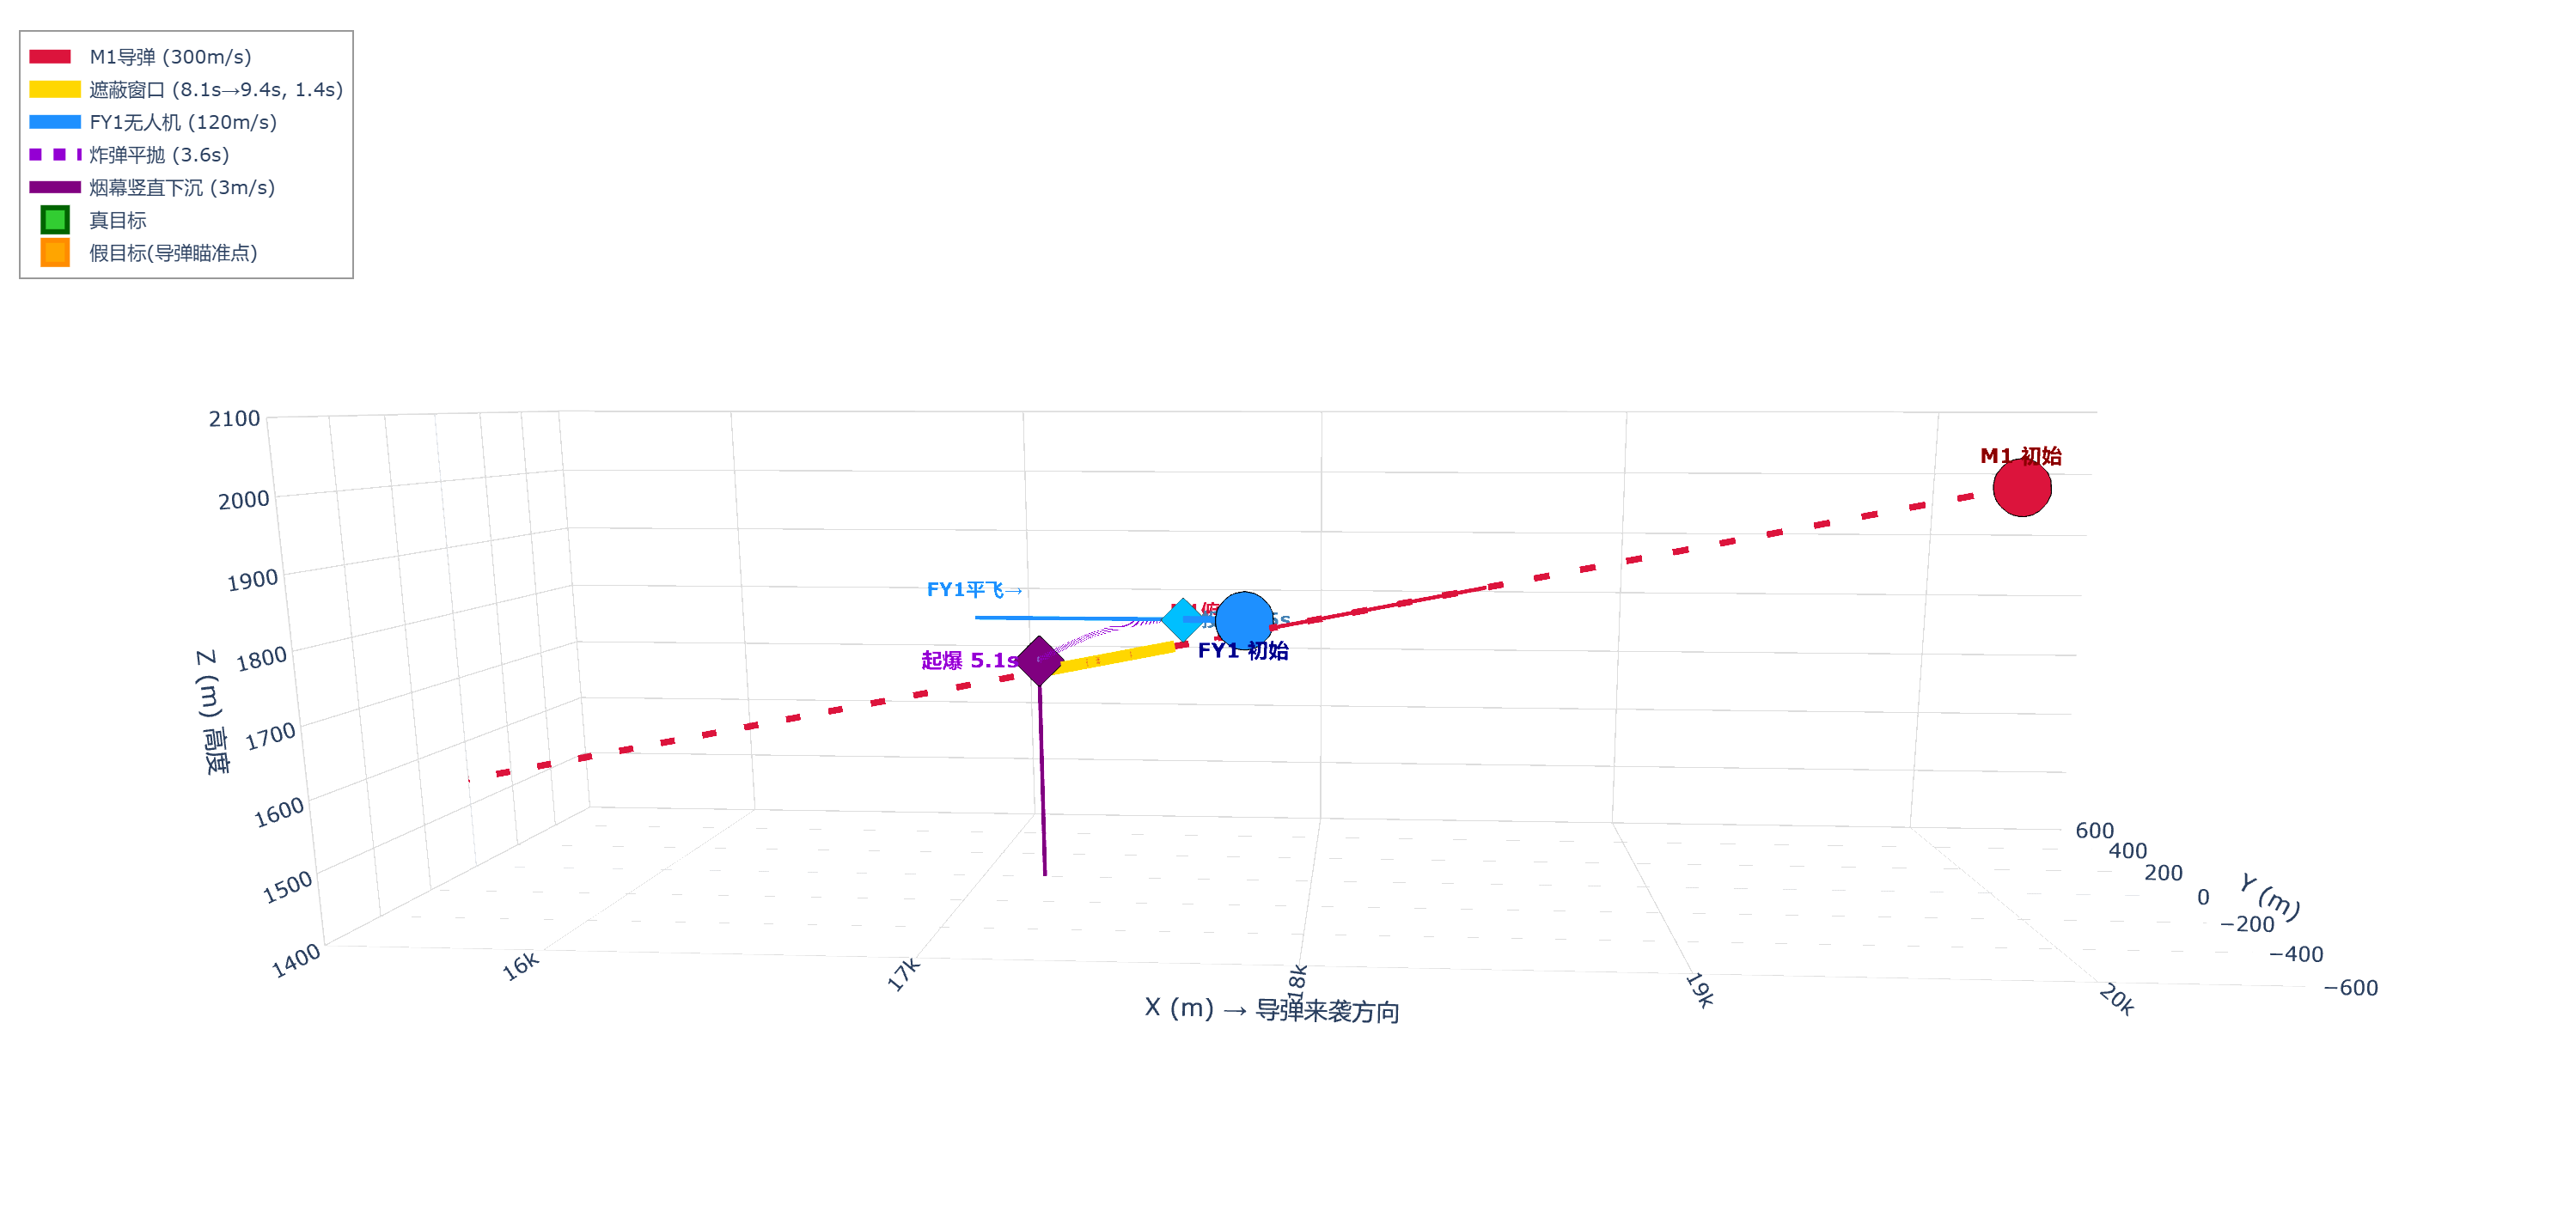
\includegraphics[width=0.8\textwidth]{20260804135851_234_32.png}
    \caption{空间轨迹和遮蔽关系}
    \label{fig:trace}
\end{figure}
\subsection{运动学模型}
\subsubsection{导弹运动方程}
导弹$M_1$初始位置$\mathbf{M}_0=(20000,0,2000)$，其速度恒定为$V_M=300\mathrm{m/s}$，且据题意，该导弹飞行方向不变，沿直线指向原点$O_d$，故其运动为匀速直线运动，运动方向的单位向量为
\[
\hat{\mathbf{u}}_m = \frac{\mathbf{O}_d - \mathbf{M}_0}{\|\mathbf{O}_d - \mathbf{M}_0\|}
= \frac{(-20000, 0, -2000)}{\sqrt{20000^2 + 2000^2}} \approx (-0.995, 0, -0.100)
\]
所以导弹的运动方程以矢量形式可表示为：
\[
\mathbf{M}(t) = \mathbf{M}_0 + \hat{\mathbf{u}}_m \cdot V_M \cdot t
\]
导弹从初始位置飞到原点需时 $T_{\text{end}} = \|\mathbf{M}_0\| / V_M = \sqrt{20000^2 + 2000^2}/300 \approx 67.1\ \mathrm{s}$。
\subsubsection{无人机与烟幕弹}
无人机$FY1$的初始位置为$\mathbf{P}_{\text{FY1}}=(17800,0,1800)$，其以恒定速度$V_{\text{drone}}=120\mathrm{m/s}$朝假目标方向做高度不变的匀速直线运动，若取该方向方向向量$\hat{\mathbf{u}}_f = (-1, 0, 0)$，受领任务后$t_{\text{rel}} = 1.5\ \mathrm{s}$ 时刻投放烟幕弹，延时$t_{\text{delay}} = 3.6\ \mathrm{s}$ 后起爆。

炸弹投放后，由于惯性在水平方向做匀速直线运动，竖直方向受重力作用做匀加速直线运动，我们取 $g = 9.8\ \mathrm{m/s^2}$ 。投放点 $\mathbf{R}_{\text{pt}}$与起爆点 $\mathbf{A}_{\text{det}}$ 的位置可以由矢量形式写为：
\[
\mathbf{R}_{\text{pt}} = \mathbf{P}_{\text{FY1}} + V_{\text{drone}} \cdot \hat{\mathbf{u}}_f \cdot t_{\text{rel}}
\]

故$\mathbf{R}_\text{pt}= (17620, 0, 1800) $
\[
\mathbf{A}_{\text{det}} = \mathbf{R}_{\text{pt}} + V_{\text{drone}} \cdot \hat{\mathbf{u}}_f \cdot t_{\text{delay}} + (0, 0, -\tfrac{1}{2} g t_{\text{delay}}^2)
\]

代入得 $\mathbf{A}_{\text{det}} = (17188, 0, 1736.5)$。

随后，烟幕弹起爆，瞬间形成一个半径$R_s=10\mathrm{m}$的球体，并以$v_s=3\mathrm{m/s}$匀速下沉，其烟幕有效遮蔽时间$T_\text{life}=20\mathrm{s}$。

起爆时刻 $t_{\text{det}} = t_{\text{rel}} + t_{\text{delay}} = 5.1\ \mathrm{s}$。烟幕球心位置的时间函数为：
\[
\mathbf{A}(t) = \mathbf{A}_{\text{det}} - (0, 0, v_s) \cdot (t - t_{\text{det}}), \quad t \in [t_{\text{det}},\; t_{\text{det}}+ T_{\text{life}}].
\]
$t < t_{\text{det}}$ 时烟幕尚未起爆，$t > t_{\text{det}} + T_{\text{life}}$ 时烟幕已失效。所以我们的目标是计算该固定投放参数下烟幕对 M1 的有效遮蔽总时长 $T_{\text{eff}}$。

为了后续求根方便，将烟幕运动改写为
\[
\mathbf{A}(t) = \tilde{\mathbf{A}}_0 - (0,0,v_s)\,t,\quad \tilde{\mathbf{A}}_0 = \mathbf{A}_{\text{det}} + (0,0,v_s)t_{\text{det}},
\]
同时导弹相对烟幕的相对运动为
\begin{equation}
\mathbf{M}(t)-\mathbf{A}(t)=\mathbf{d}_0 + \mathbf{v}_{\text{rel}}\,t,
\label{eq:rel-mot}
\end{equation}
其中
\[
\mathbf{d}_0 = \mathbf{M}_0 - \tilde{\mathbf{A}}_0,\qquad
\mathbf{v}_{\text{rel}} = \hat{\mathbf{u}}_m V_M + (0,0,v_s).
\]

\subsection{遮蔽判定与临界方程}
在模型准备中已经给出了遮蔽状态的判别式(1)，这里将其转化为临界方程以便精确求根。遮蔽状态发生切换的时刻正是以下三类方程取等号的时刻。

\subsubsection{C1 边界：导弹进入/离开烟幕球}
条件 C1 为 $\|\mathbf{M}(t)-\mathbf{A}(t)\| \le R_s$，边界方程为
\[
\|\mathbf{M}(t)-\mathbf{A}(t)\|^2 = R_s^2.
\]

将式$(2)$代入，有
\[
\|\mathbf{v}_{\text{rel}}\|^2 t^2 + 2(\mathbf{d}_0\cdot\mathbf{v}_{\text{rel}}) t +  \|\mathbf{d}_0\|^2 - R_s^2 = 0,
\]

这是一个标准的一元二次方程，我们记$a_2 = \|\mathbf{v}_{\text{rel}}\|^2$，$a_1 = 2(\mathbf{d}_0\cdot\mathbf{v}_{\text{rel}})$，$a_0 = \|\mathbf{d}_0\|^2 - R_s^2$，则方程化为
\[
a_2 t^2 + a_1 t + a_0 = 0,
\]

判别式 $\Delta = a_1^2 - 4a_2a_0$，当 $\Delta\ge 0$ 时两根为
\[
t_{\text{enter}},\;t_{\text{exit}} = \frac{-a_1 \mp \sqrt{\Delta}}{2a_2}.
\]

我们保留落在有效区间 $[t_{\text{det}}, t_{\text{det}}+T_{\text{life}}]$ 内的根，这就是导弹进入烟幕球和离开烟幕球的精确时刻。

\subsubsection{C2 边界}
C2 条件包含两个子条件：角度覆盖（条件b）和几何前置（条件a）。故对其边界分别处理。

\textbf{条件b边界}：
定义函数
\[
f_{\text{C2}}(t) = \alpha(t) - \theta_{\max}(t),
\]
其中$\alpha(t)$与$\theta_{\max}(t)$均为模型准备中定义的函数：
\[
\alpha(t)=\arcsin\!\left(\frac{R_s}{\|\mathbf{M}(t)-\mathbf{A}(t)\|}\right),
\]
\[
\theta_{\max}(t)=\max_{\mathbf{P}\in\partial\mathcal{C}_{\text{vis}}(\mathbf{M}(t))}
\arccos\!\left(
\frac{(\mathbf{P}-\mathbf{M}(t))\cdot(\mathbf{A}(t)-\mathbf{M}(t))}
{\|\mathbf{P}-\mathbf{M}(t)\|\,\|\mathbf{A}(t)-\mathbf{M}(t)\|}
\right).
\]
$f_{\text{C2}}(t)>0$ 表示角度覆盖成立。由于我们无法计算出 $f_{\text{C2}}(t)=0$的一个精确解析解，所以我们采用二分法来数值计算。具体步骤：
\begin{enumerate}
    \item 在 $[t_{\text{det}}, t_{\text{det}}+T_{\text{life}}]$ 上均匀取 40 个点，步长 $0.5\mathrm{s}$，计算 $f_{\text{C2}}$。
    \item 若相邻点函数值异号，则在该小区间内用二分法求根，精度设为 $10^{-6}\mathrm{s}$。
\end{enumerate}

\textbf{条件a边界}：
当导弹和烟幕球心与真目标等距时，C2失效，即
\[
\|\mathbf{M}(t)-O_1\|^2 = \|\mathbf{A}(t)-O_1\|^2.
\]

同样代入运动方程，整理为二次方程
\[
a_2^g t^2 + a_1^g t + a_0^g = 0,
\]

其中
\[
a_2^g = \|\hat{\mathbf{u}}_m V_M\|^2 - v_s^2,\quad
a_1^g = 2\big[(\mathbf{M}_0-O_1)\cdot(\hat{\mathbf{u}}_m V_M) + (\tilde{\mathbf{A}}_0-O_1)\cdot(0,0,v_s)\big],
\]
\[
a_0^g = \|\mathbf{M}_0-O_1\|^2 - \|\tilde{\mathbf{A}}_0-O_1\|^2.
\]

取其落在有效区间且满足 $\|\mathbf{M}-O_1\| \le \|\mathbf{A}-O_1\|$ 的根，记为 $t_{\text{geom}}$，该时刻之后烟幕已不再位于目标前方。

\subsection{问题一数值结果}
将问题一给定的参数代入上述方程，求得各临界时刻如下（表\ref{tab:p1-results}）：
\begin{table}[H]
\centering
\caption{问题一各临界时刻}
\label{tab:p1-results}
\begin{tabular}{c|c|c|c|c}
\toprule
$t_{\text{det}}$（起爆）& $t_{\text{C2\_start}}$（C2开始）& $t_{\text{C1\_enter}}$（入球）& $t_{\text{geom}}$（几何失效）& $t_{\text{C1\_exit}}$（出球）\\
\midrule
$5.100$ & $8.057$ & $9.388$ & $9.419$ & $9.449$ \\
\bottomrule
\end{tabular}
\end{table}

根据这些临界点，我们可以还原出导弹被遮蔽的全过程：
\begin{itemize}
    \item 起爆后至$8.057$s：$\alpha$不足，无遮蔽。
    \item $8.057$s至$9.388$s：角度覆盖成立（导弹在球外），时长$1.332$s。
    \item $9.388$s至$9.419$s：导弹进入烟幕球内，此时条件C1满足。
    \item $9.419$s至$9.449$s：C2条件失效，但C1条件满足，此时导弹仍在球内，仍是有效遮蔽。
    \item $9.449$s以后：导弹出球，C1失效，遮蔽结束。
\end{itemize}
因此有效遮蔽总时长
\[
T_{\text{eff}} =9.449-8.057= 1.392\ \mathrm{s}.
\]

该时长仅占导弹全程飞行时间$67.1$s的约$2.1\%$，表明在给定的固定参数下遮蔽效果十分有限，这也凸显了后续问题中开展参数优化的必要性。

\section{问题二求解}
\label{sec:p2}

问题二在问题一的基础上，将无人机航向、速度、烟幕弹投放与起爆时机作为决策变量，以最大化有效遮蔽时间 $T_{\text{eff}}$ 为目标，建立单机单弹策略优化模型。由于目标函数无解析梯度，可行域在四维空间中极为狭窄，我们采用\textbf{锚点搜索 + 局部贝叶斯优化（BO）}的两阶段策略进行求解。

\subsection{决策变量与约束条件}

烟幕弹的投放与起爆过程可由起爆时刻 $t_{\text{det}}$ 和起爆点 $\mathbf{A}_{\text{det}}=(A_x,A_y,A_z)$ 唯一确定。定义四维决策向量为
\[
\mathbf{x} = [\,t_{\text{det}},\; A_x,\; A_y,\; A_z\,] \in \mathbb{R}^4.
\]

给定 $\mathbf{x}$ 后，无人机飞行参数由逆向公式唯一确定：
\begin{align}
v(\mathbf{x}) &= \frac{\sqrt{(A_x - 17800)^2 + (A_y)^2}}{t_{\text{det}}}, \\
t_{\text{fall}}(\mathbf{x}) &= \sqrt{\frac{2(1800 - A_z)}{g}}, \quad g = 9.8\ \mathrm{m/s^2}, \\
t_{\text{rel}}(\mathbf{x}) &= t_{\text{det}} - t_{\text{fall}}.
\end{align}

约束条件：$v \in [70, 140]\ \mathrm{m/s}$，$t_{\text{rel}} \geq 0$，$A_z \in [50, 1795]\ \mathrm{m}$。目标函数 $T_{\text{eff}}(\mathbf{x})$ 沿用问题一的遮蔽判定模型（式\ref{eq:shielded}）。

\subsection{可行域稀疏性与锚点搜索}

通过 $5000$ 次随机采样验证：满足所有约束且 $T_{\text{eff}}>0$ 的命中率为 $0/5000=0\%$。可行域是四维空间中的``针尖''状极窄区域。从零开始的全局BO必然失败——GP在绝大多数采样点上只观测到常数 $T_{\text{eff}}\approx 0$，无法学到空间结构。为此采用两阶段策略：粗粒度网格 + 坐标下降精化定位锚点，再以锚点为中心进行局部 BO。

\subsubsection{粗粒度网格遍历}
由物理直觉确定搜索范围：
\[
t_{\text{det}} \in [2.0, 4.3]\ \mathrm{s},\; A_x \in [17550, 17700]\ \mathrm{m},\; A_y \in [-15, 15]\ \mathrm{m},\; A_z \in [1740, 1790]\ \mathrm{m}.
\]

各维 6 等分得 $6^4=1296$ 个节点，可行点 138 个。网格最优解为：
\[
\mathbf{x}_{\text{grid}} = [t_{\text{det}} = 2.92,\; A_x = 17550,\; A_y = 9,\; A_z = 1760], \quad T_{\text{eff}} = 4.3230\ \mathrm{s}.
\]

\subsubsection{坐标下降局部精化}
为避免Nelder-Mead在陡峭可行域边界的数值不稳定性，采用纯Python坐标下降：从网格最优解出发，沿每轴正负方向尝试移动，步长初始 $[0.05\ \mathrm{s}, 50\ \mathrm{m}, 5\ \mathrm{m}, 10\ \mathrm{m}]$，3轮后步长减半。24次评估将 $T_{\text{eff}}$ 从 $4.3230$ 提升至 $4.5244\ \mathrm{s}$（$+4.7\%$）。

最终锚点：
\[
\mathbf{x}_{\text{anchor}} = [t_{\text{det}} = 3.007,\; A_x = 17525,\; A_y = 9,\; A_z = 1760], \quad T_{\text{eff}} = 4.5244\ \mathrm{s}.
\]

反推飞行参数：$v \approx 91.5\ \mathrm{m/s}$，$\theta \approx 178.1^\circ$，$t_{\text{fall}} \approx 2.86\ \mathrm{s}$，$t_{\text{rel}} \approx 0.15\ \mathrm{s}$。无人机以中等速度沿 $-X$ 方向飞行 $3.007\ \mathrm{s}$，炸弹经 $2.86\ \mathrm{s}$ 自由落体至 $1760\ \mathrm{m}$ 起爆。对比问题一固定参数解（$T_{\text{eff}}=1.39\ \mathrm{s}$），优化后遮蔽时长提升至 $3.25$ 倍。

\subsection{高斯过程代理模型与EI采集}

锚点已定位可行区域的大致位置，但坐标下降仅沿坐标轴搜索，无法探索参数间的耦合效应（如 $t_{\text{det}}$ 与 $A_x$ 的协同调整）。需要一种方法在锚点邻域内建立目标函数的局部近似，并自动权衡``在已知高值区域精调''与``去未探索区域冒险''。高斯过程（GP）代理模型恰好满足这一需求——它不需要 $T_{\text{eff}}$ 的梯度，仅假设目标函数是``平滑''的：起爆参数相近的两个策略，遮蔽效果也相近。这一假设在物理上是自然的：$T_{\text{eff}}$ 由导弹--烟幕--目标的连续几何关系决定，不存在不连续跳变（不可行区域由惩罚函数平滑连接）。

搜索框以锚点为中心：$\mathbf{lb} = [0.5, 17250, -191, 1460]$，$\mathbf{ub} = [5.9, 17800, 209, 1790]$。拉丁超立方采样 $n_0=15$ 点，注入锚点和网格最优点建立初始GP模型。

RBF核函数：$k(\mathbf{x}, \mathbf{x}') = \sigma_f^2 \exp(-\frac{1}{2}\sum_{j=1}^{4} (x_j - x'_j)^2/\ell_j^2)$，$\ell_j = 0.2(ub_j-lb_j)$，$\sigma_f^2 = 2.0$。

后验预测：$\mu(\mathbf{x}_*) = \mathbf{k}_*^T (\mathbf{K} + \sigma_n^2\mathbf{I})^{-1}\mathbf{y}$，$\sigma^2(\mathbf{x}_*) = k(\mathbf{x}_*,\mathbf{x}_*) - \mathbf{k}_*^T(\mathbf{K} + \sigma_n^2\mathbf{I})^{-1}\mathbf{k}_*$，$\sigma_n^2 = 10^{-3}$。

期望改进采集函数：$\mathrm{EI}(\mathbf{x}) = \Delta\cdot\Phi(Z) + \sigma\cdot\phi(Z)$，$\Delta = \mu - y_{\text{best}} - 0.01$，$Z = \Delta/\sigma$。不可行策略用平滑惩罚返回负值，GP 在惩罚曲面上学到连续梯度，自然引导搜索至可行域边界。

\subsection{实验结果}

BO 经 $15+60=75$ 次评估收敛。最终结果与锚点完全一致：
\[
\mathbf{x}^*_{\text{BO}} = [t_{\text{det}} = 3.007,\; A_x = 17525,\; A_y = 9,\; A_z = 1760], \quad T_{\text{eff}}^* = 4.5244\ \mathrm{s}.
\]

扩大搜索范围至 $\mathbf{lb}=[0.5,16800,-300,1000]$，$\mathbf{ub}=[10.0,17800,300,1790]$，75 次评估后仍收敛至 $4.5244\ \mathrm{s}$。5 个不同种子的多起点 BO 均收敛至 $4.5244 \pm 0.000\ \mathrm{s}$。

\begin{table}[H]
\centering
\caption{问题二各优化方法结果汇总}
\label{tab:p2-results}
\begin{tabular}{lcccl}
\toprule
\textbf{方法} & $t_{\text{det}}$ (s) & $(A_x, A_y, A_z)$ (m) & $T_{\text{eff}}$ (s) & \textbf{评估次数} \\
\midrule
网格搜索     & 2.92 & (17550, 9, 1760) & 4.3230 & 1296 \\
坐标下降精化 & 3.007 & (17525, 9, 1760) & 4.5244 & 24 \\
局部 BO     & 3.007 & (17525, 9, 1760) & 4.5244 & 75 \\
扩大 BO     & 3.007 & (17525, 9, 1760) & 4.5244 & 75 \\
5种子 BO均值& 3.007 & (17525, 9, 1760) & $4.524\pm 0.000$ & $5\times75$ \\
\bottomrule
\end{tabular}
\end{table}

确认 $T_{\text{eff}} = 4.5244\ \mathrm{s}$ 为 FY1 单弹干扰 M1 的全局最优遮蔽时长，较问题一固定参数的 $1.39\ \mathrm{s}$ 提升 $225\%$。

\section{问题三求解}
\label{sec:p3}

问题三在问题二的基础上，将可投放烟幕弹从 1 枚扩展至 3 枚。核心约束：三枚弹共享无人机的飞行方向 $\theta$ 和速度 $v$——起爆点水平投影全部位于从 FY1 出发的同一条射线上，无法横向分散。

\subsection{决策变量与约束}

每弹拥有独立的 $t_{\text{det}}^{(i)}$ 和 $t_{\text{delay}}^{(i)}$，共 $2+3\times2=8$ 个决策变量：
\[
\mathbf{x} = [\,v,\; \theta,\; t_{\text{det}}^{(1)},\; t_{\text{delay}}^{(1)},\; t_{\text{det}}^{(2)},\; t_{\text{delay}}^{(2)},\; t_{\text{det}}^{(3)},\; t_{\text{delay}}^{(3)}\,] \in \mathbb{R}^8.
\]

新增约束：$t_{\text{det}}^{(1)} < t_{\text{det}}^{(2)} < t_{\text{det}}^{(3)}$，投放间隔 $t_{\text{rel}}^{(i+1)} - t_{\text{rel}}^{(i)} \geq 1.0\ \mathrm{s}$。

目标函数为三弹遮蔽区间的并集总长：$\mathcal{F}(\mathbf{x}) = |\bigcup_{i=1}^3 \mathcal{I}^{(i)}(\mathbf{x})|$，附加单弹超界软约束惩罚（单弹 $T_{\text{eff}}$ 不可超越问题二单弹最优 $T_{\max}=4.5244\ \mathrm{s}$，见第\ref{sec:p2}节）。

\subsection{锚点引导 + CMA-ES 联合优化}

8 维空间可行域极度稀疏。以问题二最优的 $(v^*,\theta^*)=(91.50, 178.13^\circ)$ 为锚点，Bomb1 直接部署在 P2 最优位置（$t_{\text{det}}^{(1)}=3.007$，$t_{\text{delay}}^{(1)}=2.857$）。锚点评估仅 Bomb1 贡献 $T_{\text{eff}}=4.52\ \mathrm{s}$——P2 的 $(v,\theta)$ 下 Bomb2、3 无法形成遮蔽。

\textbf{第一轮 BO 快速探索：} 经 38 次评估将并集提升至 $4.80\ \mathrm{s}$（$+6.1\%$）。BO 发现关键方向：微调 $(v,\theta)$ 至 $(94.61, 178.68^\circ)$，Bomb1 牺牲 $0.09\ \mathrm{s}$（$4.52 \to 4.43$），换取 Bomb2 获得 $[5.35,8.52]$（$3.17\ \mathrm{s}$）的遮蔽区间。

然而后续三轮 BO（170 次评估）均未能超越 $4.80\ \mathrm{s}$。根因在于 8D 空间中 GP 代理模型的退化：即使注入锚点，LHS 初始采样中仅 $1/8$ 个点可行，GP 的后验方差在整个搜索框内几乎处处相等——预测曲面退化为先验均值附近的平坦函数。Expected Improvement 此时等价于在搜索框内做纯随机探索，丧失了``利用已知高值区域''的导向能力。问题二的 BO 之所以有效，是因为 4D 锚点邻域内 GP 至少有 2 个 $\Teff>0$ 的注入点可以学习局部梯度；而 8D 空间中单锚点无法提供足够的方向信息来恢复 8 维梯度。

\textbf{第二轮 CMA-ES 精细收敛：} 协方差矩阵自适应进化策略（CMA-ES）绕过 GP 代理建模这一瓶颈——它直接维护多维正态搜索分布 $\mathcal{N}(\mathbf{m},\sigma^2\mathbf{C})$，在每代采样 $\lambda=8$ 个候选解，按截断选择（取 $\mu=4$ 个最优）更新分布参数。关键优势在于：\textbf{协方差矩阵 $\mathbf{C}$ 的更新方向只取决于候选解之间的相对排序，而非目标函数绝对值}。即使多数候选解不可行，只要少数可行解的排序信息存在，分布的均值 $\mathbf{m}$ 就能向更优区域漂移，而协方差矩阵逐步学习参数间的耦合结构（如 $v$ 增大时 $\theta$ 应如何配合调整）。

从 BO 最优解出发，初始步长 $\sigma_0=0.3$，经 3 轮共 1200 次评估收敛：$4.80 \to 5.58 \to 5.64 \to 5.65\ \mathrm{s}$。后两轮（800 次）无改进，全局步长 $\sigma$ 从 $0.17$ 衰减至 $0.05$——搜索分布已收缩至极小邻域，确认全局收敛。

\subsection{最优策略与结果}

\begin{equation}
\boxed{v^* = 95.02\ \mathrm{m/s},\quad \theta^* = 178.74^\circ}
\end{equation}

\begin{table}[H]
\centering
\caption{问题三最优三弹投放策略}
\label{tab:p3-strategy}
\begin{tabular}{c|c|c|c|c|c}
\toprule
\textbf{弹} & $t_{\text{det}}$ (s) & $t_{\text{delay}}$ (s) & $t_{\text{rel}}$ (s) & $T_{\text{eff}}$ (s) & \textbf{遮蔽区间} \\
\midrule
1 & 3.24 & 3.21 & 0.04 & 3.39 & $[3.24,\; 6.63]$ \\
2 & 4.79 & 3.30 & 1.50 & 3.33 & $[5.57,\; 8.90]$ \\
3 & 7.01 & 2.87 & 4.14 & \textbf{0} & — \\
\bottomrule
\end{tabular}
\end{table}

三弹并集：$[3.24,\; 6.63] \cup [5.57,\; 8.90] = [3.24,\; 8.90]$，$T_{\text{eff}}^{\text{total}} = 5.65\ \mathrm{s}$。对比问题二单弹最优（$4.52\ \mathrm{s}$）提升 $24.8\%$，对比问题一固定参数（$1.39\ \mathrm{s}$）提升 $306\%$。

\subsection{两弹分工与 Bomb3 失效的几何根源}

最优策略呈现``两弹分工''模式：Bomb1 以极小投放延迟（$0.04\ \mathrm{s}$，几乎起飞即投放）覆盖早期 $[3.24, 6.63]$（牺牲 P2 最优的 $1.13\ \mathrm{s}$ 换取 Bomb2 空间）；Bomb2 在 $[5.57, 8.90]$ 延伸覆盖，两区间在 $[5.57,6.63]$ 重叠 $1.06\ \mathrm{s}$ 为过渡衔接。

Bomb3（$t_{\text{det}}=7.01\ \mathrm{s}$）的 $T_{\text{eff}}$ 在 CMA-ES 全部 1200 次评估中始终为 0。其失效具有明确的几何根源：三弹水平投影均位于同一条射线。C2 遮蔽需要烟幕球心位于 $\mathbf{M}(t)$ 与 $\mathbf{O}_1$ 之间（几何前置）且满足角度覆盖条件（$\alpha \geq \theta_{\max}$）。沿此射线，$t_{\text{det}}$ 增大有两个矛盾效应——起爆点更靠近目标（有利于几何前置），但导弹飞抵时的 $\theta_{\max}$ 增大而 $\alpha$ 减小（不利于角度覆盖）。同时满足两者的 $t_{\text{det}}$ 区域仅有 2 个：Bomb1 的近 FY1 端（$t_{\text{det}}\in[2.5,3.5]$）和 Bomb2 的远 FY1 端（$t_{\text{det}}\in[4.5,6.0]$）。Bomb3 的 $t_{\text{det}}\in[6.5,12.0]$ 位于两区域之外——角度条件始终不满足。

弹数增至 3 倍而遮蔽时长仅增 $25\%$，边际回报显著递减。根因在于共享航线将所有炸弹约束于同一条射线——这是单机多弹策略的固有物理上限。

\section{问题四求解}
\label{sec:p4}

问题四考察三架无人机 FY1、FY2、FY3 各投放 1 枚烟幕弹协同干扰 M1。与问题三的本质区别：每架无人机拥有独立的 $(v_i,\theta_i)$，三条航线可从不同起点出发、从不同角度接近导弹路径。

\subsection{决策变量与协同目标}

三机总决策变量为 12 维：$\mathbf{x} = [\mathbf{x}^{(1)},\mathbf{x}^{(2)},\mathbf{x}^{(3)}] \in \mathbb{R}^{12}$，每机 4 维 $\mathbf{x}^{(i)} = [t_{\text{det}}^{(i)}, A_{x,i}, A_{y,i}, A_{z,i}]$。各机独立满足与第\ref{sec:p2}节相同的约束（速度 $v_i\in[70,140]\ \mathrm{m/s}$，投放时刻非负，起爆高度合理）。三架无人机的起点与飞行高度（表\ref{tab:drone-config}）：

\begin{table}[H]
\centering
\caption{问题四无人机配置}
\label{tab:drone-config}
\begin{tabular}{c|c|c|c}
\toprule
\textbf{编号} & \textbf{起点 $(x_0, y_0)$} & \textbf{高度 $H$ (m)} & \textbf{速度范围 (m/s)} \\
\midrule
FY1 & $(17800, 0)$    & 1800 & $[70, 140]$ \\
FY2 & $(12000, 1400)$ & 1400 & $[70, 140]$ \\
FY3 & $(6000, -3000)$ & 700  & $[70, 140]$ \\
\bottomrule
\end{tabular}
\end{table}

协同目标函数为三弹遮蔽区间并集总长：$T_{\text{eff}}^{\text{joint}} = |\bigcup_{i=1}^3 \mathcal{I}^{(i)}|$。导弹飞行时间约束 $T_{\text{flight}} \approx 67.0\ \mathrm{s}$：导弹到达假目标后烟幕失效，遮蔽区间上限被截断至 $\min(t_{\text{det}}+T_{\text{life}}, T_{\text{flight}})$。

\subsection{三阶段分层求解策略}

12 维可行域极其稀疏——三架无人机各自 4D``针尖''的笛卡尔积。从零开始的全局优化不可能命中联合可行域。采用三阶段分级策略逐层缩小搜索范围。

\textbf{Phase 0 —— 物理引导锚点搜索：} FY1 直接复用问题二最优解（$T_{\text{eff}}=4.52\ \mathrm{s}$）。对 FY2 和 FY3，利用几何必要条件——起爆点应位于 $\mathbf{M}(t_{\text{det}})\to\mathbf{O}_1$ 连线附近——进行物理引导采样：对候选 $t_{\text{det}}$，在连线邻域随机撒点作为起爆位置。FY2 经 12000 次采样获锚点 $T_{\text{eff}}=2.37\ \mathrm{s}$，FY3 用 108 点确定性网格获锚点 $T_{\text{eff}}=1.21\ \mathrm{s}$。

\textbf{Phase 1 —— BO 单机精化：} FY3 经 GP+EI（$n_0=30$，$N=100$）将 $T_{\text{eff}}$ 从 $1.21$ 提升至 $2.96\ \mathrm{s}$（$+144\%$）。FY2 因锚点搜索可行率极低（$2/12000$），BO 未能显著改进。

\textbf{Phase 2 —— CMA-ES 联合优化：} Phase 1 的独立 BO 不考虑区间重叠（三枚弹分别优化时互不知晓对方的存在），直接将独立最优拼接未必能得到好的联合并集——实际上，初始拼接解的 $T_{\text{eff}}^{\text{joint}}$ 为负惩罚值（FY2 的 Phase 1 锚点不可行）。需要在 12D 联合空间中进行协同优化。此处直接使用 CMA-ES 而非 BO——理由与第\ref{sec:p3}节一致：12D 空间中 GP 的代理建模比 8D 更加困难（可行域是三个 4D``针尖''的笛卡尔积），而 CMA-ES 的排序驱动更新不依赖全局代理模型，只要分布均值保持在可行域附近，搜索就能持续改进。CMA-ES（$\lambda=6$，300 次评估）成功将 FY2 从不可行区引导至可行，并协同微调三机参数消除区间重叠。

\subsection{最优协同策略}

\begin{table}[H]
\centering
\caption{问题四最优协同投放策略}
\label{tab:p4-strategy}
\begin{tabular}{c|c|c|c|c|c|c}
\toprule
\textbf{无人机} & $t_{\text{det}}$ (s) & $t_{\text{rel}}$ (s) & $(A_x, A_y, A_z)$ (m) & $T_{\text{eff}}$ (s) & $v$ (m/s) & $\theta$ ($^\circ$) \\
\midrule
FY1 & 2.86 & 0.05  & (17525, 8, 1761) & 4.52 & 96.1  & 178.3 \\
FY2 & 24.92 & 14.88 & (9003, 51, 906)  & 3.34 & 131.9 & 204.2 \\
FY3 & 29.16 & 26.21 & (6495, 78, 657)  & 2.97 & 106.9 & 80.9 \\
\bottomrule
\end{tabular}
\end{table}

三弹遮蔽区间完全无重叠，形成完美的时空接力：
\[
\boxed{\mathcal{I}_{\text{joint}} = [3.54,\; 8.06] \cup [24.92,\; 28.26] \cup [29.78,\; 32.75],\quad T_{\text{eff}}^{\text{joint}} = 10.83\ \mathrm{s}}
\]

\subsection{时空分层的物理图景}

三架无人机在时间、空间、高度三个维度形成立体接力体系：

\begin{enumerate}
    \item \textbf{时间分层：} FY1 早期（$[3.5,8.1]\ \mathrm{s}$，导弹距目标 $\sim19\ \mathrm{km}$）$\to$ FY2 中段（$[24.9,28.3]\ \mathrm{s}$，距目标 $\sim12\ \mathrm{km}$）$\to$ FY3 中后段（$[29.8,32.8]\ \mathrm{s}$，距目标 $\sim9\ \mathrm{km}$）。三段在时间轴上错开分布，互不重叠。
    \item \textbf{空间分层：} FY1 从 $X=17800$ 出发覆盖前端，FY2 从 $X=12000$ 覆盖中段，FY3 从 $X=6000$ 覆盖后端。三者在 $X$ 轴沿导弹飞行路径形成前--中--后的接力链。
    \item \textbf{高度分层：} FY1 在 $1761\ \mathrm{m}$ 高空起爆（遮蔽大俯角视线），FY2 在 $906\ \mathrm{m}$ 中空起爆，FY3 在 $657\ \mathrm{m}$ 低空起爆（遮蔽近水平视线）。烟幕从高到低对真目标圆柱体形成立体遮蔽覆盖。
\end{enumerate}

\subsection{协同增益分析}

\begin{table}[H]
\centering
\caption{各问题遮蔽时长横向对比}
\label{tab:comparison}
\begin{tabular}{lcc}
\toprule
\textbf{指标} & \textbf{数值} & \textbf{说明} \\
\midrule
问题一基准       & 1.39 s  & 固定参数计算 \\
问题二单弹最优   & 4.52 s  & FY1 单机基准 \\
问题三三弹协同   & 5.65 s  & 单机三弹（共享航线）\\
问题四三机协同   & \textbf{10.83 s} & 三机各一弹（独立航线）\\
覆盖率           & 16.2\%  & $10.83/67.0$ \\
vs 问题二        & \textbf{2.39}$\times$ & 三机独立航线增益 \\
vs 问题三        & \textbf{1.92}$\times$ & 空间自由度增益 \\
\bottomrule
\end{tabular}
\end{table}

多机独立航线的空间自由度是遮蔽时长从 $5.65\ \mathrm{s}$ 跃升至 $10.83\ \mathrm{s}$ 的根本原因。三条航线可从不同角度、不同高度、不同时段拦截导弹，形成自然的时空分工——这是单机多弹（问题三）受共享航线约束所无法实现的。

\end{document}
